% $Id: template.tex 11 2007-04-03 22:25:53Z jpeltier $

\documentclass{vgtc}                          % final (conference style)
% \documentclass[review]{vgtc}                 % review
%\documentclass[widereview]{vgtc}             % wide-spaced review
%\documentclass[preprint]{vgtc}               % preprint
% \documentclass[electronic]{vgtc}             % electronic version

%% Uncomment one of the lines above depending on where your paper is
%% in the conference process. ``review'' and ``widereview'' are for review
%% submission, ``preprint'' is for pre-publication, and the final version
%% doesn't use a specific qualifier. Further, ``electronic'' includes
%% hyperreferences for more convenient online viewing.

%% Please use one of the ``review'' options in combination with the
%% assigned online id (see below) ONLY if your paper uses a double blind
%% review process. Some conferences, like IEEE Vis and InfoVis, have NOT
%% in the past.

%% Figures should be in CMYK or Grey scale format, otherwise, colour 
%% shifting may occur during the printing process.

%% These three lines bring in essential packages: ``mathptmx'' for Type 1 
%% typefaces, ``graphicx'' for inclusion of EPS figures. and ``times''
%% for proper handling of the times font family.

\usepackage{mathptmx}
\usepackage{graphicx}
\usepackage{color}
\usepackage{times}
\usepackage{xargs}                      % Use more than one optional parameter in a new commands
\usepackage[pdftex,dvipsnames]{xcolor}  % Coloured text etc.
\usepackage[hidelinks]{hyperref}
\usepackage{listings}
\usepackage{float}
\usepackage{lipsum}
\usepackage{enumitem}
\newfloat{lstfloat}{htb}{lop} % p flag deactivated
\floatname{lstfloat}{Listing}

\newcommand\blfootnote[1]{%
  \begingroup
  \renewcommand\thefootnote{}\footnote{#1}%
  \addtocounter{footnote}{-1}%
  \endgroup
}

% TODO notes
\setlength {\marginparwidth }{1.5cm}
\usepackage[colorinlistoftodos,prependcaption,textsize=tiny]{todonotes}
\newcommandx{\unsure}[2][1=]{\todo[linecolor=red,backgroundcolor=red!25,bordercolor=red,#1]{#2}}
\newcommandx{\change}[2][1=]{\todo[linecolor=blue,backgroundcolor=blue!25,bordercolor=blue,#1]{#2}}
\newcommandx{\info}[2][1=]{\todo[linecolor=OliveGreen,backgroundcolor=OliveGreen!25,bordercolor=OliveGreen,#1]{#2}}
\newcommandx{\improvement}[2][1=]{\todo[linecolor=Plum,backgroundcolor=Plum!25,bordercolor=Plum,#1]{#2}}
\newcommandx{\thiswillnotshow}[2][1=]{\todo[disable,#1]{#2}}
\usepackage[utf8]{inputenc}
\usepackage[labelfont={bf},textfont={bf},font=small]{caption}
\usepackage[labelfont={bf},textfont={bf},font=small]{subcaption} % if two images are rigth next to eachother

%\let\ifpdf\relax
%% unknown extension .eps instead
%\usepackage{epstopdf}

%% We encourage the use of mathptmx for consistent usage of times font
%% throughout the proceedings. However, if you encounter conflicts
%% with other math-related packages, you may want to disable it.

%% If you are submitting a paper to a conference for review with a double
%% blind reviewing process, please replace the value ``0'' below with your
%% OnlineID. Otherwise, you may safely leave it at ``0''.
\onlineid{0}

%% declare the category of your paper, only shown in review mode
\vgtccategory{Research}

%% allow for this line if you want the electronic option to work properly
\vgtcinsertpkg

%% In preprint mode you may define your own headline.
%\preprinttext{To appear in an IEEE VGTC sponsored conference.}

%% Paper title.

\title{Exploring the Expediency of Multiclass Density Maps}

%% This is how authors are specified in the conference style

%% Author and Affiliation (single author).
\author{Tobias Lahmann\thanks{e-mail: tobias.lahmann@uni-ulm.de}}
\affiliation{\scriptsize Universit\"at Ulm}

%% Author and Affiliation (multiple authors with single affiliations).
%%\author{Roy G. Biv\thanks{e-mail: roy.g.biv@aol.com} %
%%\and Ed Grimley\thanks{e-mail:ed.grimley@aol.com} %
%%\and Martha Stewart\thanks{e-mail:martha.stewart@marthastewart.com}}
%%\affiliation{\scriptsize Martha Stewart Enterprises \\ Microsoft Research}

%% Author and Affiliation (multiple authors with multiple affiliations)
% \author{Tobias Lahmann\thanks{e-mail:tobias.lahmann@uni-ulm.de}\\ %
%      \scriptsize Universit\"at Ulm %
% \and Christian van Onzenoodt\thanks{e-mail:christian.van-onzenoodt@uni-ulm.de}\\ %
%      \scriptsize Universit\"at Ulm %
% \and Timo Ropinski\thanks{e-mail:timo.ropinski@uni-ulm.de}\\ %
%      \scriptsize Universit\"at Ulm %
% }

%% A teaser figure can be included as follows, but is not recommended since
%% the space is now taken up by a full width abstract.
%\teaser{
%  \includegraphics[width=1.5in]{sample.eps}
%  \caption{Lookit! Lookit!}
%}

%% Abstract section.
\begin{abstract}
	This document is a model and instructions for \LaTeX.
	This and the IEEEtran.cls file define the components of your paper [title, text, heads, etc.]. *CRITICAL: Do Not Use Symbols, Special Characters, Footnotes, 
	or Math in Paper Title or Abstract.
\end{abstract}

%% ACM Computing Classification System (CCS). 
%% See <http://www.acm.org/class/1998/> for details.
%% The ``\CCScat'' command takes four arguments.

\CCScatlist{ 
  \CCScat{H.5.2}{Information Interfaces and Presentation}{User Interfaces}{Evaluation/methodology}
  % \CCScat{E.1}{Data}{Data Structures}{Graphs and networks}
}

%% Copyright space is enabled by default as required by guidelines.
%% It is disabled by the 'review' option or via the following command:
% \nocopyrightspace

%%%%%%%%%%%%%%%%%%%%%%%%%%%%%%%%%%%%%%%%%%%%%%%%%%%%%%%%%%%%%%%%
%%%%%%%%%%%%%%%%%%%%%% START OF THE PAPER %%%%%%%%%%%%%%%%%%%%%%
%%%%%%%%%%%%%%%%%%%%%%%%%%%%%%%%%%%%%%%%%%%%%%%%%%%%%%%%%%%%%%%%%

\begin{document}

\section{Introduction}

In the field of software development there are some keywords like security, consistency or reliability that are indispensable today. Everyone wants the best and most intelligent software, but with increasing complexity the possibility of fault-proneness in the software increases. In the following, the aforementioned topic is examined under the programming language model of object orientation and metrics that can be considered, which is an important topic in research trends in software technology nowadays.
One might think that testing the software and the resulting errors is one of the last steps in the software development process, but this is a false assumption. The earlier the system is examined and tested for critical points, the more work will be saved in later, more cost-intensive development steps.

A software fault is defined as an anomalous condition or defect at the component, device, or subsystem level that can lead to a failure. Therefore an undesirable companion of developing, where the objective is to appear as little as possible.
Fault-proneness is an important external software quality attribute of interest to software developers and practitioners. The fault-proneness of an object-oriented class indicates the extent to which the class, given the metrics for that class, is fault-prone. Since it is difficult to measure the fault-proneness of software that is not yet in use, predictive models are applied to estimate the fault-proneness of software classes.

Several studies like "\textit{Fault-Proneness of Open Source Software: Exploring its Relations to Internal Software Quality and Maintenance Process}" \cite{kozlov2013fault} or "\textit{Empirical analysis for investigating the effect of object-oriented metrics on fault proneness: a replicated case study}" \cite{b2aggarwal2009empirical} have been carried out to determine which metrics are useful in capturing important quality attributes such as fault-proneness  and fault prediction, which are summarized in the following sections.
Furthermore the main research objective is the consolidation of some metrics and methods related to fault-proneness in the software development process.

This paper is organized as follows: Section \ref{content} deals with the content background of design metrics in object-oriented systems and the basic technologies about object orientation. In Section \ref{research} the research methodology is described. Afterwards the Section \ref{related} presents some studies and further literature that handle the concept of fault prediction and further analysis in that topic area. After the related work, it comes to the Section \ref{analysis}, that contains the analysis and summary of obejct-oriented design metrics and the results of some empirical studies that are concerned with fault-proneness and that used to support the software development process. After the investigation of the effects on these metrics, a discussion follows in Section \ref{discussion}, including the classification of the relevance in the software development process and the parties involved.Furthermore there are limitations and benefits of the considered metrics. Finally, the paper is concluded and gives an outlook in Section \ref{conclusion}.

% \section{Exposition}

\textcolor{red}{
	Lorem ipsum dolor sit amet, consetetur sadipscing elitr, sed diam nonumy eirmod tempor invidunt ut labore et dolore magna aliquyam erat, sed diam voluptua. At vero eos et accusam et justo duo dolores et ea rebum. Stet clita kasd gubergren, no sea takimata sanctus est Lorem ipsum dolor sit amet. Lorem ipsum dolor sit amet, consetetur sadipscing elitr, sed diam nonumy eirmod tempor invidunt ut labore et dolore magna aliquyam erat, sed diam voluptua. At vero eos et accusam et justo duo dolores et ea rebum. Stet clita kasd gubergren, no sea takimata sanctus est Lorem ipsum dolor sit amet. Lorem ipsum dolor sit amet, consetetur sadipscing elitr, sed diam nonumy eirmod tempor invidunt ut labore et dolore magna aliquyam erat, sed diam voluptua. At vero eos et accusam et justo duo dolores et ea rebum. Stet clita kasd gubergren, no sea takimata sanctus est Lorem ipsum dolor sit amet.}

\textcolor{red}{
	Duis autem vel eum iriure dolor in hendrerit in vulputate velit esse molestie consequat, vel illum dolore eu feugiat nulla facilisis at vero eros et accumsan et iusto odio dignissim qui blandit praesent luptatum zzril delenit augue duis dolore te feugait nulla facilisi. Lorem ipsum dolor sit amet, consectetuer adipiscing elit, sed diam nonummy nibh euismod tincidunt ut laoreet dolore magna aliquam erat volutpat.}

\textcolor{red}{
	Ut wisi enim ad minim veniam, quis nostrud exerci tation ullamcorper suscipit lobortis nisl ut aliquip ex ea commodo consequat. Duis autem vel eum iriure dolor in hendrerit in vulputate velit esse}

\begin{figure}
	\centering
	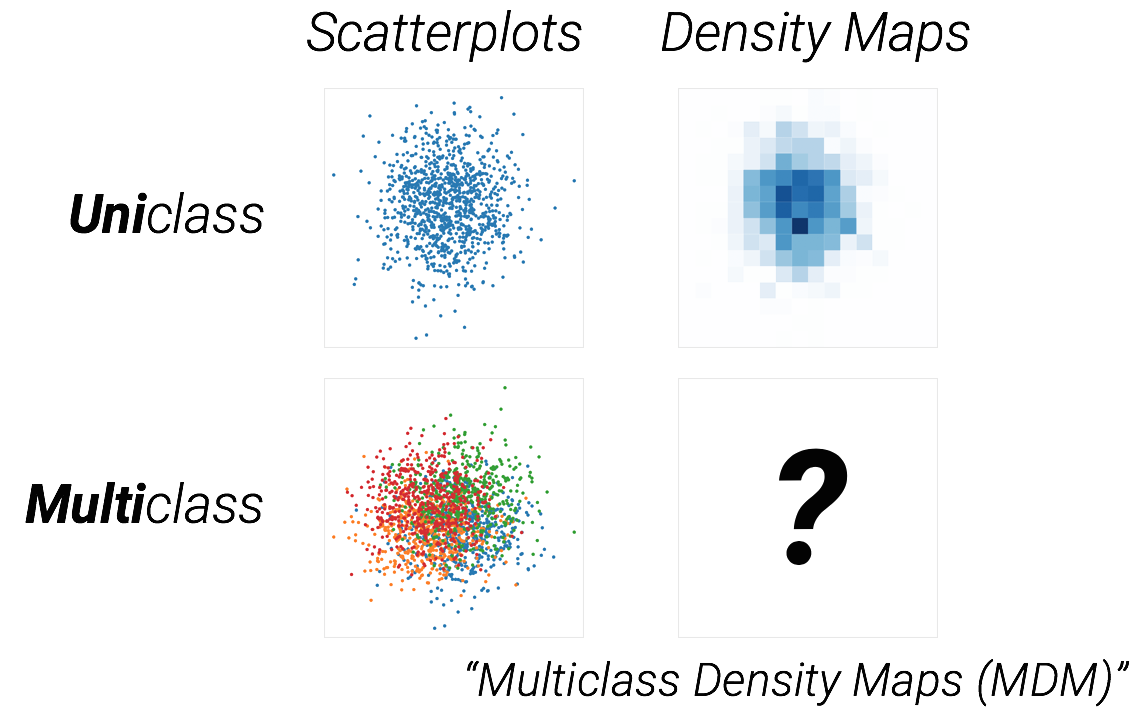
\includegraphics[width=0.9\columnwidth]{./figures/motivation}
	\caption[motivation]{The different scatterplot types. MDM is multiclass and a density map. \textcolor{red}{Lorem ipsum dolor sit amet, consetetur sadipscing elitr, sed diam nonumy eirmod tempor invidunt ut labore et dolore magna aliquyam erat, sed diam voluptua. At vero eos et accusam et justo duo dolores et ea rebum.}}~\label{fig:motivation}
\end{figure}

\textcolor{red}{
	Lorem ipsum dolor sit amet, consetetur sadipscing elitr, sed diam nonumy eirmod tempor invidunt ut labore et dolore magna aliquyam erat, sed diam voluptua. At vero eos et accusam et justo duo dolores et ea rebum. Stet clita kasd gubergren, no sea takimata sanctus est Lorem ipsum dolor sit amet. Lorem ipsum dolor sit amet, consetetur sadipscing elitr, sed diam nonumy eirmod tempor invidunt ut labore et dolore magna aliquyam erat, sed diam voluptua. At vero eos et accusam et justo duo dolores et ea rebum. Stet clita kasd gubergren, no sea takimata sanctus est Lorem ipsum dolor sit amet. Lorem ipsum dolor sit amet, consetetur sadipscing elitr, sed diam nonumy eirmod tempor invidunt ut labore et dolore magna aliquyam erat, sed diam voluptua. At vero eos et accusam et justo duo dolores et ea rebum. Stet clita kasd gubergren, no sea takimata sanctus est Lorem ipsum dolor sit amet.}

\textcolor{red}{
	Duis autem vel eum iriure dolor in hendrerit in vulputate velit esse molestie consequat, vel illum dolore eu feugiat nulla facilisis at vero eros et accumsan et iusto odio dignissim qui blandit praesent luptatum zzril delenit augue duis dolore te feugait nulla facilisi. Lorem ipsum dolor sit amet, consectetuer adipiscing elit, sed diam nonummy nibh euismod tincidunt ut laoreet dolore magna aliquam erat volutpat.}

\textcolor{red}{
	Ut wisi enim ad minim veniam, quis nostrud exerci tation ullamcorper suscipit lobortis nisl ut aliquip ex ea commodo consequat. Duis autem vel eum iriure dolor in hendrerit in vulputate velit esse}

\begin{equation}
	\sum_{j=1}^{z} j = \frac{z(z+1)}{2}
\end{equation}

\begin{figure}
	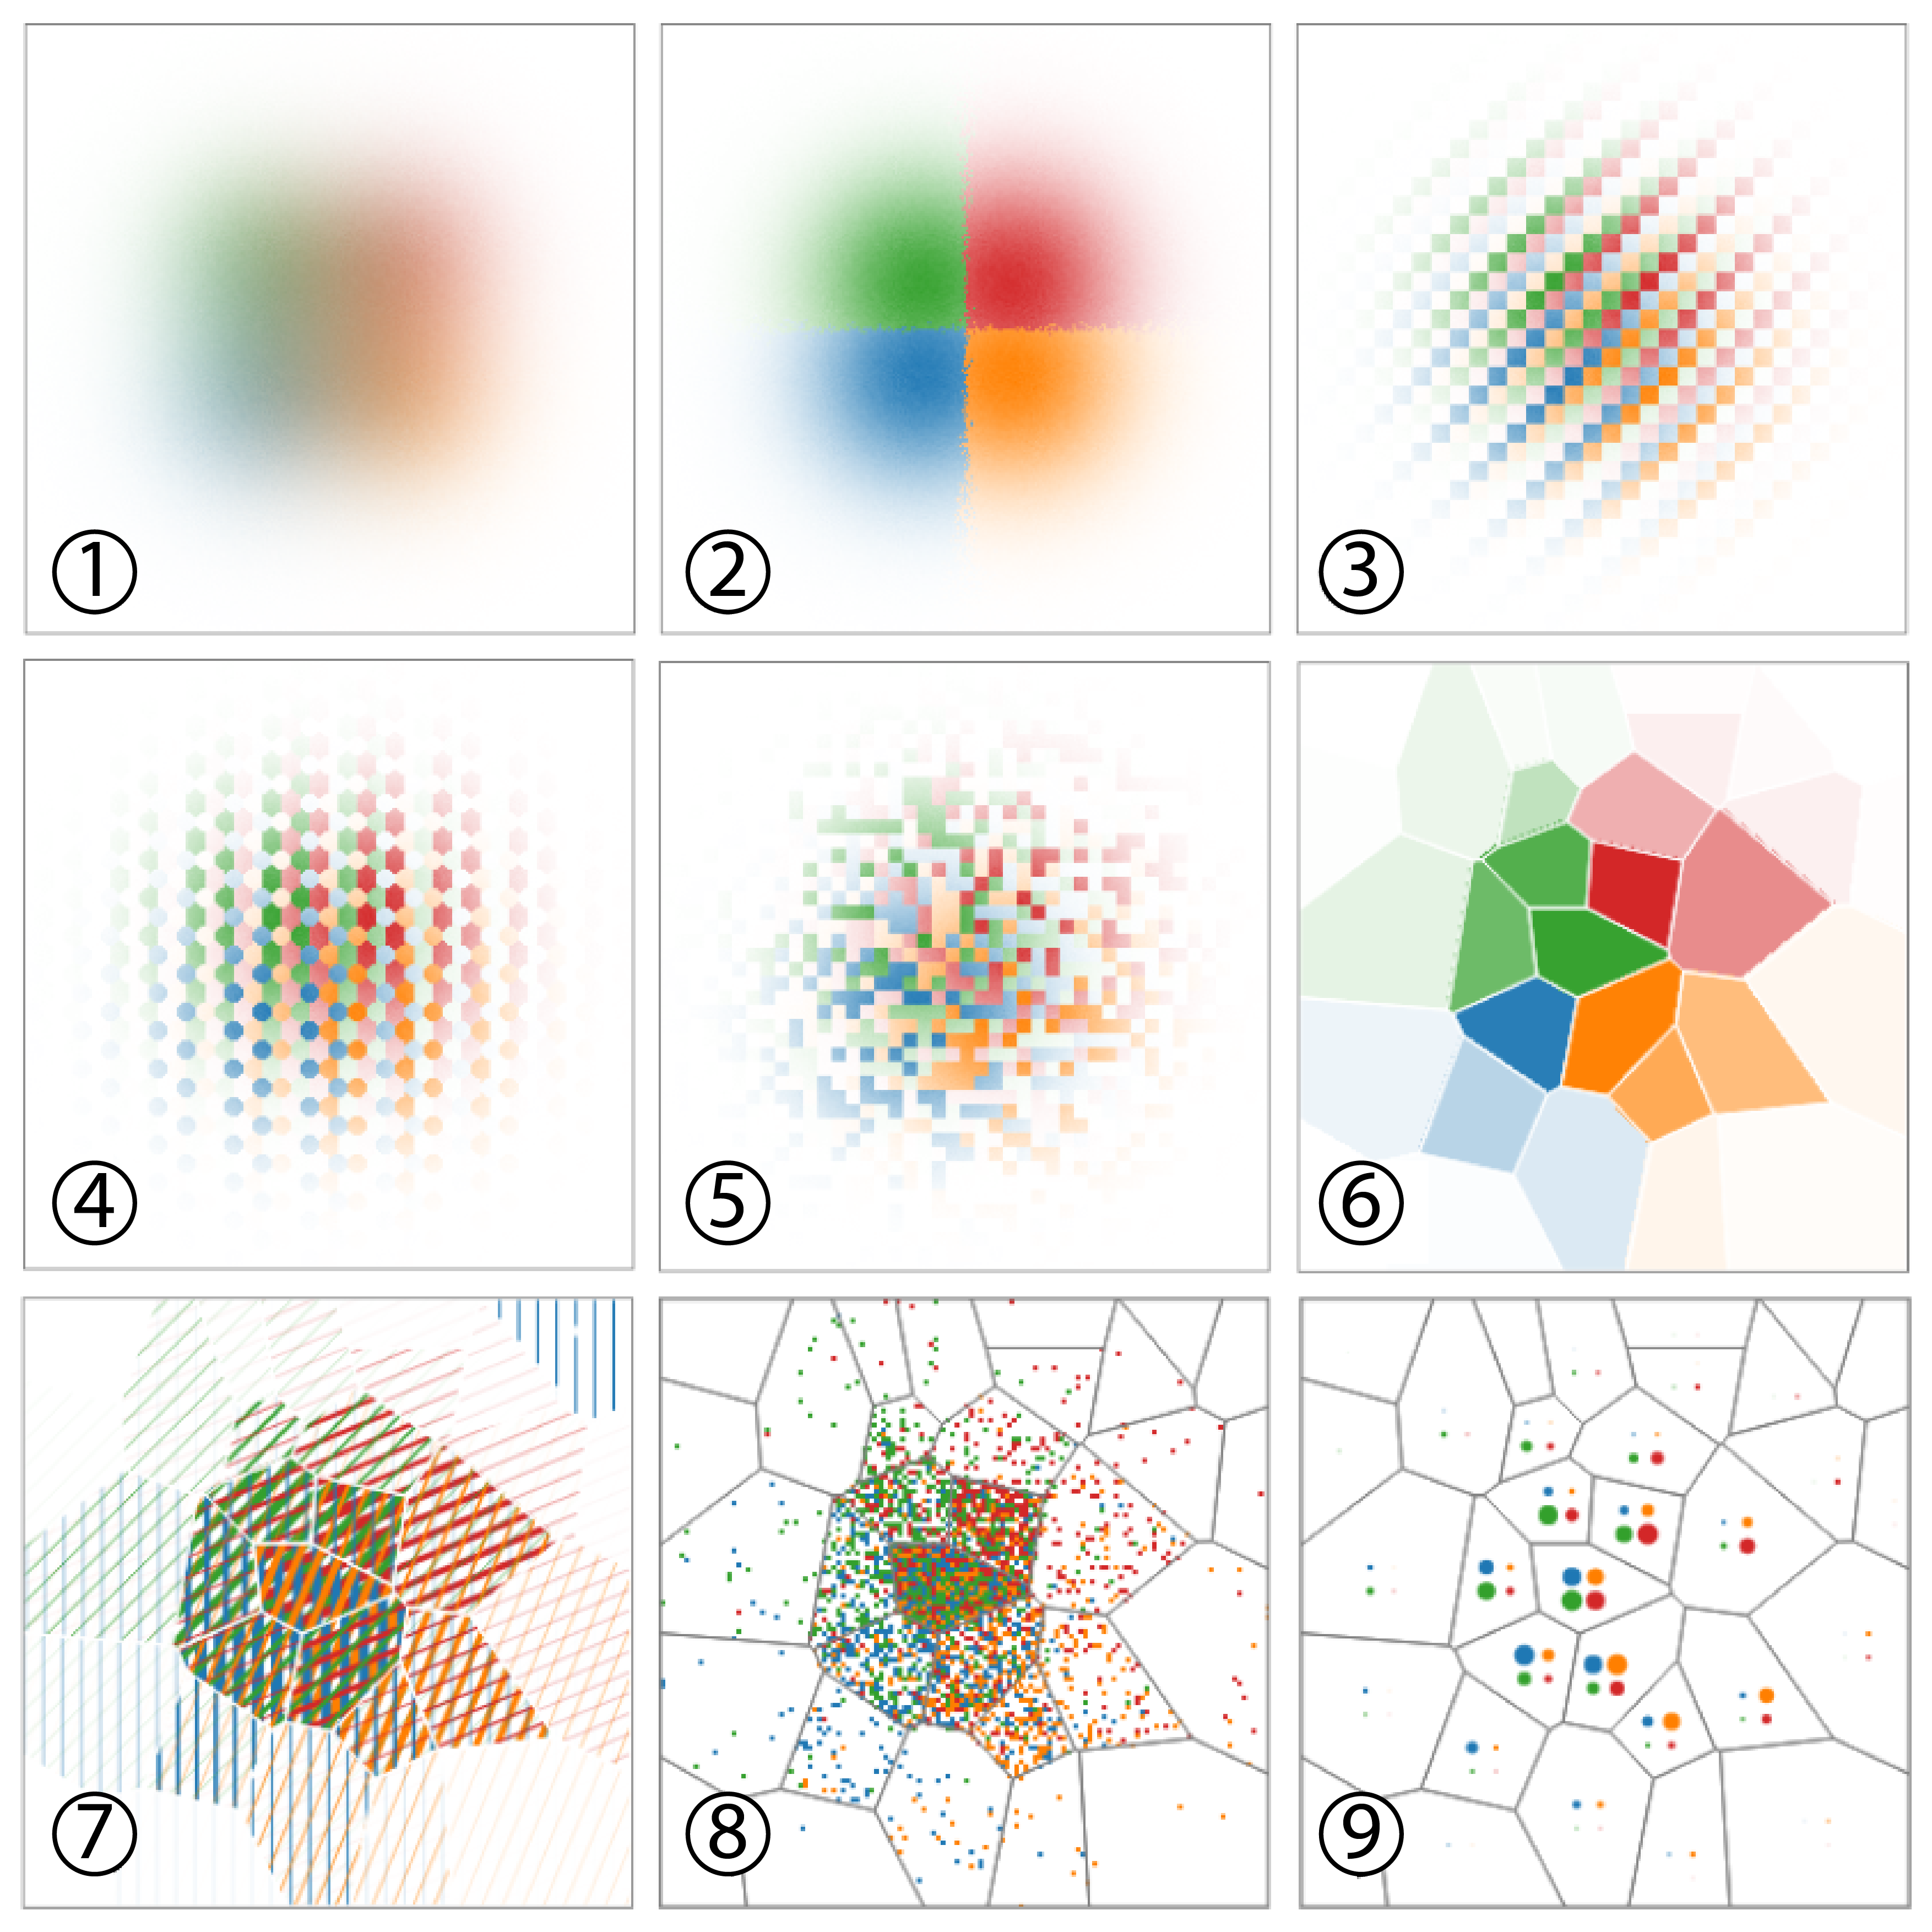
\includegraphics[width=\columnwidth]{./figures/results}
	\caption{A few results generated from the Class Buffer model. \textcolor{red}{Lorem ipsum dolor sit amet, consetetur sadipscing elitr, sed diam nonumy eirmod tempor invidunt ut labore et dolore magna aliquyam erat, sed diam voluptua. At vero eos et accusam et justo duo dolores et ea rebum.}}\label{fig:mdm-results}
\end{figure}

\textcolor{red}{
	Lorem ipsum dolor sit amet, consetetur sadipscing elitr, sed diam nonumy eirmod tempor invidunt ut labore et dolore magna aliquyam erat, sed diam voluptua. At vero eos et accusam et justo duo dolores et ea rebum. Stet clita kasd gubergren, no sea takimata sanctus est Lorem ipsum dolor sit amet. Lorem ipsum dolor sit amet, consetetur sadipscing elitr, sed diam nonumy eirmod tempor invidunt ut labore et dolore magna aliquyam erat, sed diam voluptua. At vero eos et accusam et justo duo dolores et ea rebum. Stet clita kasd gubergren, no sea takimata sanctus est Lorem ipsum dolor sit amet. Lorem ipsum dolor sit amet, consetetur sadipscing elitr, sed diam nonumy eirmod tempor invidunt ut labore et dolore magna aliquyam erat, sed diam voluptua. At vero eos et accusam et justo duo dolores et ea rebum. Stet clita kasd gubergren, no sea takimata sanctus est Lorem ipsum dolor sit amet.}

% \begin{table}
%   \caption{Vis Paper Acceptance Rate}
%   \label{vis_accept}
%   \scriptsize
%   \begin{center}
%     \begin{tabular}{cccc}
%       Year & Submitted & Accepted & Accepted (\%)\\
%     \hline
%       1994 &  91 & 41 & 45.1\\
%       1995 & 102 & 41 & 40.2\\
%       1996 & 101 & 43 & 42.6\\
%       1997 & 117 & 44 & 37.6\\
%       1998 & 118 & 50 & 42.4\\
%       1999 & 129 & 47 & 36.4\\
%       2000 & 151 & 52 & 34.4\\
%       2001 & 152 & 51 & 33.6\\
%       2002 & 172 & 58 & 33.7\\
%       2003 & 192 & 63 & 32.8\\
%       2004 & 167 & 46 & 27.6\\
%       2005 & 268 & 88 & 32.8\\
%       2006 & 228 & 63 & 27.6
%     \end{tabular}
%   \end{center}
% \end{table}

%\begin{figure}[htb]
%  \centering
%  \includegraphics[width=1.5in]{sample.eps}
%  \caption{Sample illustration.}
%\end{figure}

% \subsection{Mezcal Head}

% Duis autem~\cite{Lorensen:1987:MCA} vel eum iriure dolor in hendrerit
% in vulputate velit esse molestie consequat, vel illum dolore eu
% feugiat nulla facilisis at vero eros et accumsan et iusto odio
% dignissim qui blandit praesent luptatum zzril delenit augue duis
% dolore te feugait nulla facilisi. Lorem ipsum dolor sit amet,
% consectetuer adipiscing elit, sed diam nonummy nibh euismod tincidunt
% ut laoreet dolore magna aliquam erat volutpat%
% \footnote{Footnotes appear at the bottom of the column}.


% \subsubsection{Ejector Seat Reservation}

% Ut wisi enim ad minim veniam, quis nostrud exerci tation ullamcorper
% suscipit lobortis nisl ut aliquip ex ea commodo
% consequat~\cite{Nielson:1991:TAD}. Duis autem vel eum iriure dolor in
% hendrerit in vulputate velit esse molestie consequat, vel illum dolore
% eu feugiat nulla facilisis at vero eros et accumsan et iusto odio
% dignissim qui blandit praesent luptatum zzril delenit augue duis
% dolore te feugait nulla facilisi.

% \paragraph{Rejected Ejector Seat Reservation}

% Ut wisi enim ad minim veniam, quis nostrud exerci tation ullamcorper
% suscipit lobortis nisl ut aliquip ex ea commodo consequat. Duis autem
% vel eum iriure dolor in hendrerit in vulputate velit esse molestie


\section{Related Work}\label{related}

To take a close look at fault-proneness in object oriented systems, basic object orientation knowledge is important, as explained in section \ref{content}. The paper "\textit{Beyond Language Independent Object-Oriented Metrics: Model Independent Metrics}" \cite{lanza2002beyond} deals not only with the concept of object orientation but also beyond languages and paradigms. The aspects of object orientation such as class, method and attribute can be found as shown in the following tables, which are subdivided into individual metrics. The model from figure \ref{fig0} serves as a template to understand the relationships between the individual metrics. 

In the following tables \ref{tab:classmetrics},\ref{tab:methodmetrics} and \ref{tab:attributesmetrics} the abbrevations and the associated metrics are listed. The used model and the metrics of the tables allow a multiple extension into different research directions. Thus, they fit the principle of object orientation and serve as a basic template to get into the basic structure of metrics. The advantages of this approach are the increased flexibility, i.e., new metamodels can be introduced from any context (for example, the financial world or databases), which provides a standard metric without the need to implement new metrics every time a new context is introduced \cite{lanza2002beyond}. Now, if you look at this system completely from an object orientation perspective, you can see that the basic programming concepts are translated into metrics. Each new method or variable crates more space to generate faults. The complexity of a class is depends, i.e., on the number of methods (NOM) or the number of attributes (NOA), that can be calculated with $NOA = NIV + NCV$, as shown in table \ref{tab:classmetrics}. An important metric about the methods of a class is the number of input parameters (NOP) or the number of access on attributes (NMAA), as you can see in figure \ref{tab:methodmetrics}. For the attribute metrics, the number of direct hits is of great importance, as can be found in figure \ref{tab:attributesmetrics}. 

\begin{table}
	\caption{Class metrics from the meta model.}~\label{tab:classmetrics}
	
	\setlength\tabcolsep{3pt}
	\renewcommand{\arraystretch}{1.4}% for the vertical padding
	\begin{tabularx}{\columnwidth}{ | c | p{7cm} | }
		\hline
		Abbrevation & Description \\ \hline\hline
		HNL & Number of classes in superclass chain of class \\ \hline
		NAM & Number of abstract methods \\ \hline
		NCV & Number of class variables \\ \hline
		NIA & Number of inherited attributes \\ \hline
		NIV & Number of instance variables \\ \hline
		NME & Number of methods extended, i.e., redefined in subclass by invoking the same method on a superclass \\ \hline	
		NMI & Number of methods inherited, i.e., defined in superclass and inherited unmodified by subclass\\ \hline
		NMO & Number of methods overridden, i.e., redefined compared to superclass\\ \hline
		NOA & Number of attributes $(NOA = NIV + NCV)$ \\ \hline
		NOC & Number of immediate subclasses of a class \\ \hline
		NOM & Number of methods\\ \hline
		PriA & Number of private attributes (equivalent for protected and public attributes)\\ \hline
		PriM & Number of private methods (equivalent for protected and public attributes)\\ \hline
		WLOC & Sum of all lines of codes over all methods \\ \hline
		WMSG & Sum of message sends in a class\\ \hline
		WNMAA & Number of all accesses on attributes\\ \hline
		WNOC & Number of all descendant classes\\ \hline
		WNOS & Sum of statements in all method bodies of class\\ \hline
		WNI & Number of invocations of all methods \\ \hline
	\end{tabularx}
\end{table}

\begin{table}
	\caption{Method metrics from the meta model.}~\label{tab:methodmetrics}
	
	\setlength\tabcolsep{3pt}
	\renewcommand{\arraystretch}{1.4}% for the vertical padding
	\begin{tabularx}{\columnwidth}{ | c | p{7cm} | }
		\hline
		Abbrevation & Description \\ \hline\hline
		LOC & Method lines of code \\ \hline
		NMA & Number of methods added, i.e., defined in subclass and not in superclass \\ \hline
		MSG & Number of method messages send \\ \hline
		NOP & Number of input parameters \\ \hline
		NI & Number of invocations of other methods within method body \\ \hline
		NMAA & Number of access on attributes \\ \hline
		NOS & Number of statements in method body \\ \hline
	\end{tabularx}
\end{table}

\begin{table}
	\caption{Attribute metrics from the meta model.}~\label{tab:attributesmetrics}
	
	\setlength\tabcolsep{3pt}
	\renewcommand{\arraystretch}{1.4}% for the vertical padding
	\begin{tabularx}{\columnwidth}{ | c | p{7cm} | }
		\hline
		Abbrevation & Description \\ \hline\hline
		AHNL & Class HNL in which attribute is defined \\ \hline
		NAA & Number of times directly accessed \\ \hline
	\end{tabularx}
\end{table}

Many metrics used in various studies are reflected in the tables.
The limitations of this approach are that not all object-oriented software metrics can be defined in terms of the language independent model, but these metrics serve as a basic overview. Certain metrics tend to be very specialized and are therefore difficult to define in a generic way. Another limitation of this basic concept is that for some metrics, there is it is not yet known how best to define them in a generic way, so the meta model does not include coupling metrics and cohesion metrics.

In another paper, a systematic literature review was reviewed that looked at 106 papers published between 1991 and 2011.
Object-oriented metrics (49\%) were used almost twice as often as traditional source code metrics (27\%) or process metrics (24\%). Object-oriented and process-oriented metrics were reported to be more successful in finding bugs compared to traditional size and complexity metrics \cite{b7radjenovic2013software}. The results of the literature review show that an inheritance and an export coupling metric are strongly associated with fault-proneness. Some evidence also suggests that there may be a small number of metrics that are strongly associated with fault-proneness, and that good predictive accuracy and quality estimation accuracy can be achieved with them.

Today's evidence suggests that most faults in software applications are found in a small percentage of software components \cite{b10el2001prediction}. This means that if these faulty software components can be identified early in the lifecycle of the development project, mitigation measures can be taken, such as redesign or refactoring. For object-oriented applications, predictive models using design metrics can be used to identify faulty classes early on \cite{b10el2001prediction}. The next step is to look at related work based on the metrics just presented and expansions of those. 

In the "\textit{Fault-Proneness of Open Source Software: Exploring its Relations to
Internal Software Quality and Maintenance Process}" \cite{kozlov2013fault} study, it was investigated how the fault-proneness of open source software (OSS) can be explained in terms of internal quality attributes and metrics of the maintenance process. A total of 342 releases of these systems were studied and, as usual, software quality was considered as a set of internal and external quality attributes. A total of 76 internal quality attributes were measured and 23 maintenance process metrics were included in this study. The strengths of this study is the comparison of a few software technology trends like fault-proneness and maintainability, as well as the study itself. First the study considers a wide range of metrics than common studies. Furthermore more OOS systems were involved in order to get a better indication of the results. In addition they focused on the fault-proneness of modern Java-based systems and investigated them as an aggregated sample. The framework for assessing the maintenance process was adopted from their previous studies. The results of the factor analysis performed showed that the metrics studied can be interpreted in terms of two factors, one of which is the system size, as shown in Figure \ref{figSize}. Previous studies in this area are based only on relatively small sets of OSS systems and releases, despite the fact that OSS projects are very diverse and heterogeneous \cite{kozlov2013fault}. Conclusively, the results may not be generalizable due to their relatively limited nature. Here, larger systems were chosen and size was found to play an important aspect in fault-proneness. In many other studies only small software systems were considered and it is noticeable that many in their conclusion note that a limitation of their work is that the statements can only be applied to small sized systems \cite{kozlov2013fault, b7radjenovic2013software}.

\begin{figure}[htbp]
	\centerline{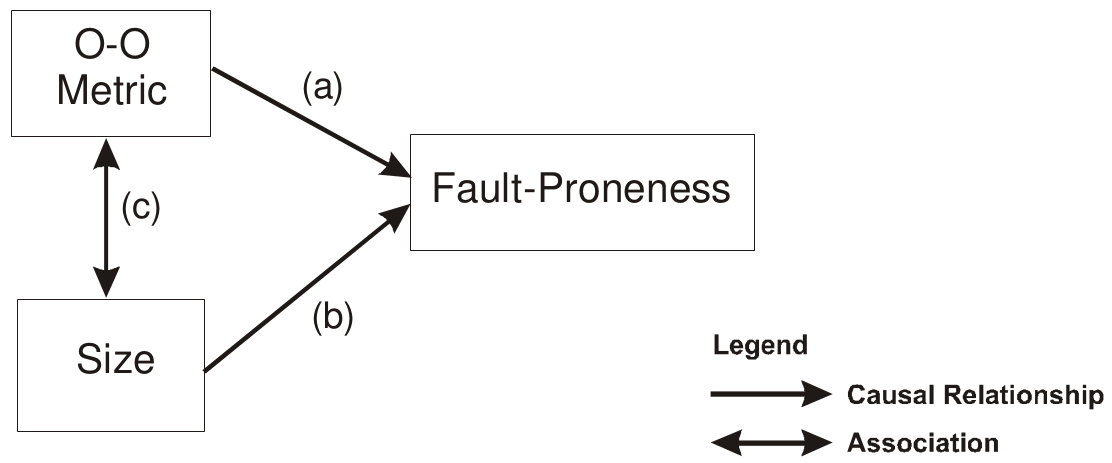
\includegraphics[width=0.45\textwidth]{pictures/faultyclasses2.png}}
	\caption{Path diagram illustrating the confounding effect of class size on the relationship between an object-oriented metric and fault-proneness \cite{b10el2001prediction}.}
	\label{figSize}
\end{figure}

Another study, also dealt with object-oriented design metrics for Java applications and construct a prediction model. It became clear that an export coupling metric exhibited the strongest association with fault-proneness, indicating a structural feature that may be symptomatic of a class with a high probability of latent faults \cite{b10el2001prediction}.

A theoretical basis for developing quantitative models that relate object-oriented metrics and external quality metrics is summarized in Figure \ref{figCoupling}. As already mentioned, one of the strongest association with fault-proneness was an export coupling metric in a study. This illustrates that there is a presumed relationship between object-oriented metrics and fault-proneness due to the effect on cognitive complexity \cite{b10el2001prediction}. Cognitive complexity can be defined as the mental load of the individuals who have to interact with the component, for example, the developers, testers, inspectors, and maintainers. 

\begin{figure}[htbp]
	\centerline{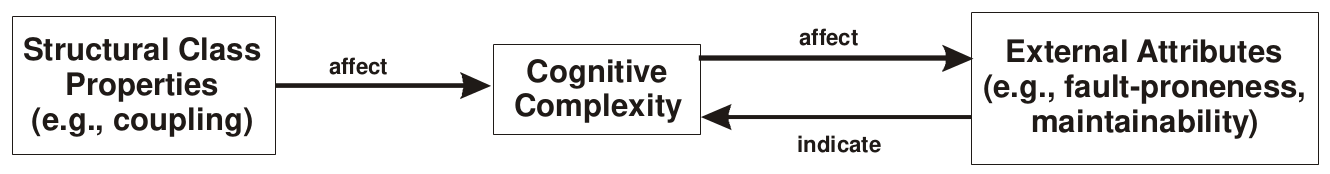
\includegraphics[width=0.5\textwidth]{pictures/faultyclasses1.png}}
	\caption{Theoretical basis for the development of object oriented product metrics \cite{b10el2001prediction}.}
	\label{figCoupling}
\end{figure}

Some studies also suggest that the depth of inheritance has an impact on the comprehensibility of object-oriented applications, and therefore would be expected to have a detrimental effect on fault-proneness \cite{b10el2001prediction}.
It was also found that inheritance leads to distributed class descriptions. That is, in this case, the complete description for a class can only be assembled by examining both the class itself and each of the superclasses of it.
Since different classes are described in different places in the code of a software program, also often distributed over several files, a programmer must turn to several places, in order to receive a complete description of a class. While this argument applies to software source code, it is not difficult to generalize it to design documents. Faults are therefore very distributed and usually cannot be found and fixed in a single place without making other changes.

Another study has considered a used set of ten software product metrics related to the following software attributes: the size of the software, coupling, cohesion, inheritance, and reuse \cite{yu2002predicting}. Some hypotheses regarding fault-proneness were empirically tested in a case study examining the client side of a large network service management system. The system under consideration is written in Java and consists of 123 classes. Validation was performed using two data analysis techniques: regression analysis and discriminant analysis.

Among other things, Class cohesion is a key attribute used to assess the design quality of a class and refers to the extent to which the methods and attributes of a class are related. Typically, classes contain special types of methods, such as constructors, destructors, and access methods, where each of these special methods has its own properties that can affect the measurement of class cohesion \cite{b4al2012impact}. Here we see again that the metrics can all be derived from the tables \ref{tab:classmetrics} and \ref{tab:methodmetrics} below.

Another paper empirically examines this impact of methods on cohesion measures. Twenty existing class cohesion metrics were used and Two types of special methods were considered, constructors and access methods. The empirical study applies the metrics, to five open source systems under four different scenarios, including first considering all special methods, second ignoring only constructors, third ignoring only access methods, and fourth ignoring all special methods.
The results of the empirical investigations show that the cohesion values for most of the considered metrics differ significantly in the four scenarios, but do not significantly affect the abilities of the metrics to predict faulty classes \cite{b4al2012impact}.

Based on this research, two more specific metrics have now been picked out, that try to support the software development process with their metrics. All of them work in their own way and in certain states of development. 
In order to provide guidance on how to proceed in the software process, some special metrics will be explained in detail now.


%A Validation of Object-Oriented Design Metrics as Quality Indicators ::: his paper presents the results of a study in which we empirically investigated the suite of object-oriented design metrics introduced in. More specifically, our goal is to assess these metrics as predictors of fault-prone classes and, therefore, determine whether they can be used as early quality indicators. This study is complementary to the work described in [30] where the same suite of metrics had been used to assess frequencies of maintenance changes to classes \cite{b11basili1996validation}.



%Assessing the Applicability of Fault-Proneness Models Across Object-Oriented Software Projects ::: Furthermore a number of papers have investigated the relationships between metrics of design and the metrics that detect faults in object oriented software. One of the main objectives of this paper is to assess whether fault-proneness models, based on design measurement, are applicable and can be viable decision making tools when applied from one object-oriented system to the other, in a given environment. \cite{b12riand2002assessing}.



%- kritische auseinandersetzung, für welche fälle sind welche metriken gut und wieso
%- Wann setz ich welche Metriken ein wann im SW Prozess!! und was kann da eintreten passieren
%- Auswirkungen von fehlern
 
%\cite{b7radjenovic2013software}. Context: Software metrics may be used in fault prediction models to improve software quality by predicing fault location. wo wie viele genutzt werden udn so

\section{Taxonomy of Separation and Perception}

With the previous work of creating effective and efficient algorithms for DR a lack of guidance for the user of certain models or algorithms has occurred~\cite{sedlmair2012taxonomy,friendly2005early}. The question how and to what extend a user can be supported and shown what DR and VE techniques to use is a non-trivial task~\cite{sedlmair2012taxonomy}.

The DimStiller system uses a workflow structure to guide users through the process of choosing DE and VE techniques~\cite{ingram2010dimstiller}, but automatic algorithms to provide such guidance have not yet emerged. To service this goal Sedlmair et al. used visual cluster separation measures~\cite{sips2009selecting, tatu2009combining}, originally developed for selecting good views within \underline{s}catter\underline{pl}ot \underline{m}atricies (SPLOM), to provide guidance for DR and VE technique choices. Two particular measures have been identified as the most effective: the \textbf{centroid} and the \textbf{grid} measure~\cite{tatu2010visual}. These names where chosen by Sedlmair et al. for readability and have been named other by different researchers~\cite{sedlmair2012taxonomy}.

They further showed that these measures fail to produce reliable results, meaning it resulted in a mismatch between the algorithms results and the quality judgement made by a person~\cite{sedlmair2012taxonomy}. The two cases of false positives and false negatives occurred; either the algorithm showed that a distinct measure was sufficient for a convincing separation to happen, but the human judged the visual separation as poor, or the algorithm failed to provide such separation but humans were indeed able to distinguish clusters in scatterplots.

These measures can be used in multiclass density maps to select the tiling, the separation of data into tiles, and thus enhance the visual impression.

% \info{two human investigators evaluated separation factors}

\subsection{Visual Cluster Separation Factors}

The general idea behind all existing separation measures is to evaluate how "pure" the neighborhoods of a scatterplot's data points are. If neighborhoods include points from many different classes they are intermixed, if only one class then they are pure~\cite{aupetit2016sepme}.
The general concept to differentiate between clusters remain generally the same and differ only based on the definitions of a neighborhood around points. Based on the work of Aupetit et al. the two definitions chosen are~\cite{aupetit2016sepme}:

\begin{itemize}[leftmargin=*]
	\setlength\itemsep{0.1em}
	\item measures with \textit{hard-neighborhoods} looks at a specific subset of the data points close to the one under focus
	\item measures with a \textit{soft-neighborhood} use the weighting of all the data points with respect to a focus point.
\end{itemize}

Local class-purity values are averaged over all possible focus points. This gives a higher purity when the local neighborhood class-purity is high for a large set of focal points, resulting in a good separation of clusters.

The separation of classes in scatterplots and density maps is dependent on different features of the plot. Participants of a study conducted by van Onzenoodt et al. indicate that spread and density of scatterplots have influence on the perception of clusters~\cite{van2017evaluating}.
When viewing scatterplots or density maps these factors are not calculated based on the mentioned approaches but rather the visual perception of clusters. This is based on each persons subjective perception of correlation and clusters~\cite{rensink2010perception, beyth1982perception, tatu2010visual}. This process can be supported by design. When the designers of maps construct the plot numerous approaches can be taken to enhance the desired effects. Some points of reference, amongst others, include count, size or density as can be seen in Figure~\ref{fig:separation_factors}. Design choices result in the improved comprehension of scatterplots and density maps.

Because multiclass scatterplots and density maps have a class property with items that need to be distinguishable, Figure~\ref{fig:separation_factors} focuses on the factors that enhance this nature and neglects within-class factors. Between-Class factors encapsulate the variance and combination of Within-Class factors across multiple classes. These factors are not described here because of the multiclass viewpoint in multiclass density maps. In the Scale section of Figure~\ref{fig:separation_factors}, the \textit{count} factor is the ratio between the number of classes and the number of points of the dataset. Sedlmair et al. found that fewer classes and many points was easier to perceive than the case of many classes, few points~\cite{sedlmair2012taxonomy}. \\
The first factor \textit{variance of density} is the mutual product of \textit{variance of size} and \textit{variance of count}. In plots where a big class is overlapping a smaller class the latter one might be identified more easily because of the law of proximity from common Gestalt psychology~\cite{kim2008object}. This is a result of a dense class being easily identifiable over sparse data.\\
The variance of shape factor ranges from similar shapes for all clusters to very different shapes across each cluster. When applied to density maps one shape might be applied to one class of data points. This will result in a mixture of shapes across the plot where a fine distinction needs to be done for the shape to be easily distinguishable to all other shapes used in the plot~\cite{borgo2013glyph, demiralp2014learning}.\\
% \textcolor{red}{\lipsum[1]}\improvement{Wtire about Demiralp et al.}
The inner-outer position in the position category describes a positional relationship between classes where a inner class can be surrounded by outer classes. Sedlmair et al. distinguish between \textit{existent} and \textit{non-existent} relations~\cite{sedlmair2012taxonomy}. They further showed that inner classes were more difficult to identify, especially those in the synthetic-gaussian data family. This shows that density maps must countermeasure this behavior with correct design adaptations.

The overarching factor is class separation. In data plots with two well separated, round, and contiguous clusters, data separation can be strongly influenced by nearly every other factor~\cite{sedlmair2012taxonomy}. For density maps the separation of classes could be the most viable factor to countermeasure the effects mentioned, mixing and masking, where data gets overlaid by other properties. In these kinds of maps it might not always be possible to apply sufficient class separation without sophisticating the two dimensional properties so designers must reside to different measures like axis scaling or using endorsed color schemes.

All of these factors can more or less be applied to multiclass density maps and the Class Buffer model, where the most significant difference is the work done before plotting the data.

\begin{figure}
	\centering
	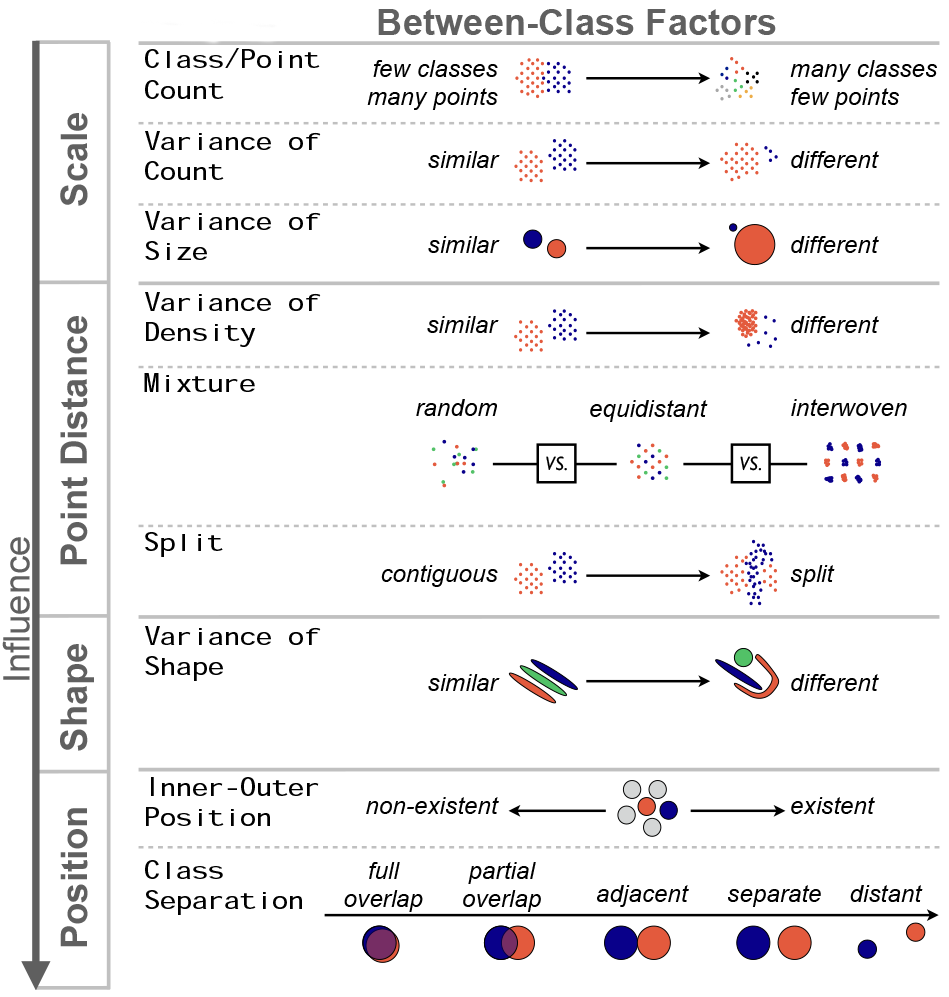
\includegraphics[width=\columnwidth]{./figures/separation}
	\caption[Separation Factors]{A taxonomy of data characteristics with respect to class separation in scatterplots. Some factors are organized as axes (arrows) while others are binned. Factors at the top can strongly influence factors below them. Class Separation is therefore dependent on all other factors.}~\label{fig:separation_factors}
\end{figure}

\subsection{Perception of Classes an Outliers}

How well different points of data are perceived in the scatterplot and density maps is a relevant task for any group of data, or even individual points. Micallef et al. focused on classes and outliers when investigating the perception within plots~\cite{micallef2017towards}.
They employ structural similarity~\cite{wang2004image} to measure the perceivability of a group of points. Structural similarity is a highly reliable image quality assessment model often applied to measure the similarity between two images~\cite{micallef2017towards}. Details on this algorithm can be taken from Wang et al.~\cite{wang2004image}.
The mean structural similarity as implemented in scikit-image~\cite{van2014scikit} can be used an applied to parts of the data with non-zero opacity. In the case of two scatterplots a and b the mean structural similarity $SSIM(a;b)$ returns values between 0 and 1, where 1 denotes that images a and b are identical.
In a case where the data of two scatterplots are almost identical but one map has a group of data points that the other one does not have, structural similarity can be taken to measure the perceived similarity between these two plots. If they are rather similar, the group of points is difficult to perceive. If the two scatterplots are rather different, then the group of points is easy to perceive~\cite{micallef2017towards}.

Overall, once users are familiar with the visualized data, they find it less difficult to perceive clusters~\cite{van2017evaluating}. Users could thus be trained to perceive classes more easily when applying similar design patterns to plots. Further, when users view multiple scatterplots or density maps they might get better at understanding these.
% \cite{aupetit2016sepme,sedlmair2012taxonomy, rensink2010perception,micallef2017towards}


\section{The Class Buffer Model}

As a result of the challenges in the perception of classes and the separation of clusters the designers of maps face various tasks to convey the correct idea to support their data. A cluster has to be well fitted into the graph to show the information in a comprehensible way. These problems can be considered each on their own but also intertwined as a whole. This is where the class buffer model comes to action.

In many approaches the designers have to think of different data aggregation, dimension reduction, visual encoding or rendering methods and know the advantages of many. The challenge of visualizing different approaches beforehand to have a mental image when creating density maps lead to the implementation of the Class Buffer model. This model takes the designer through a interactive approach to visualize data in multiclass density maps.

\begin{figure}
  \centering
	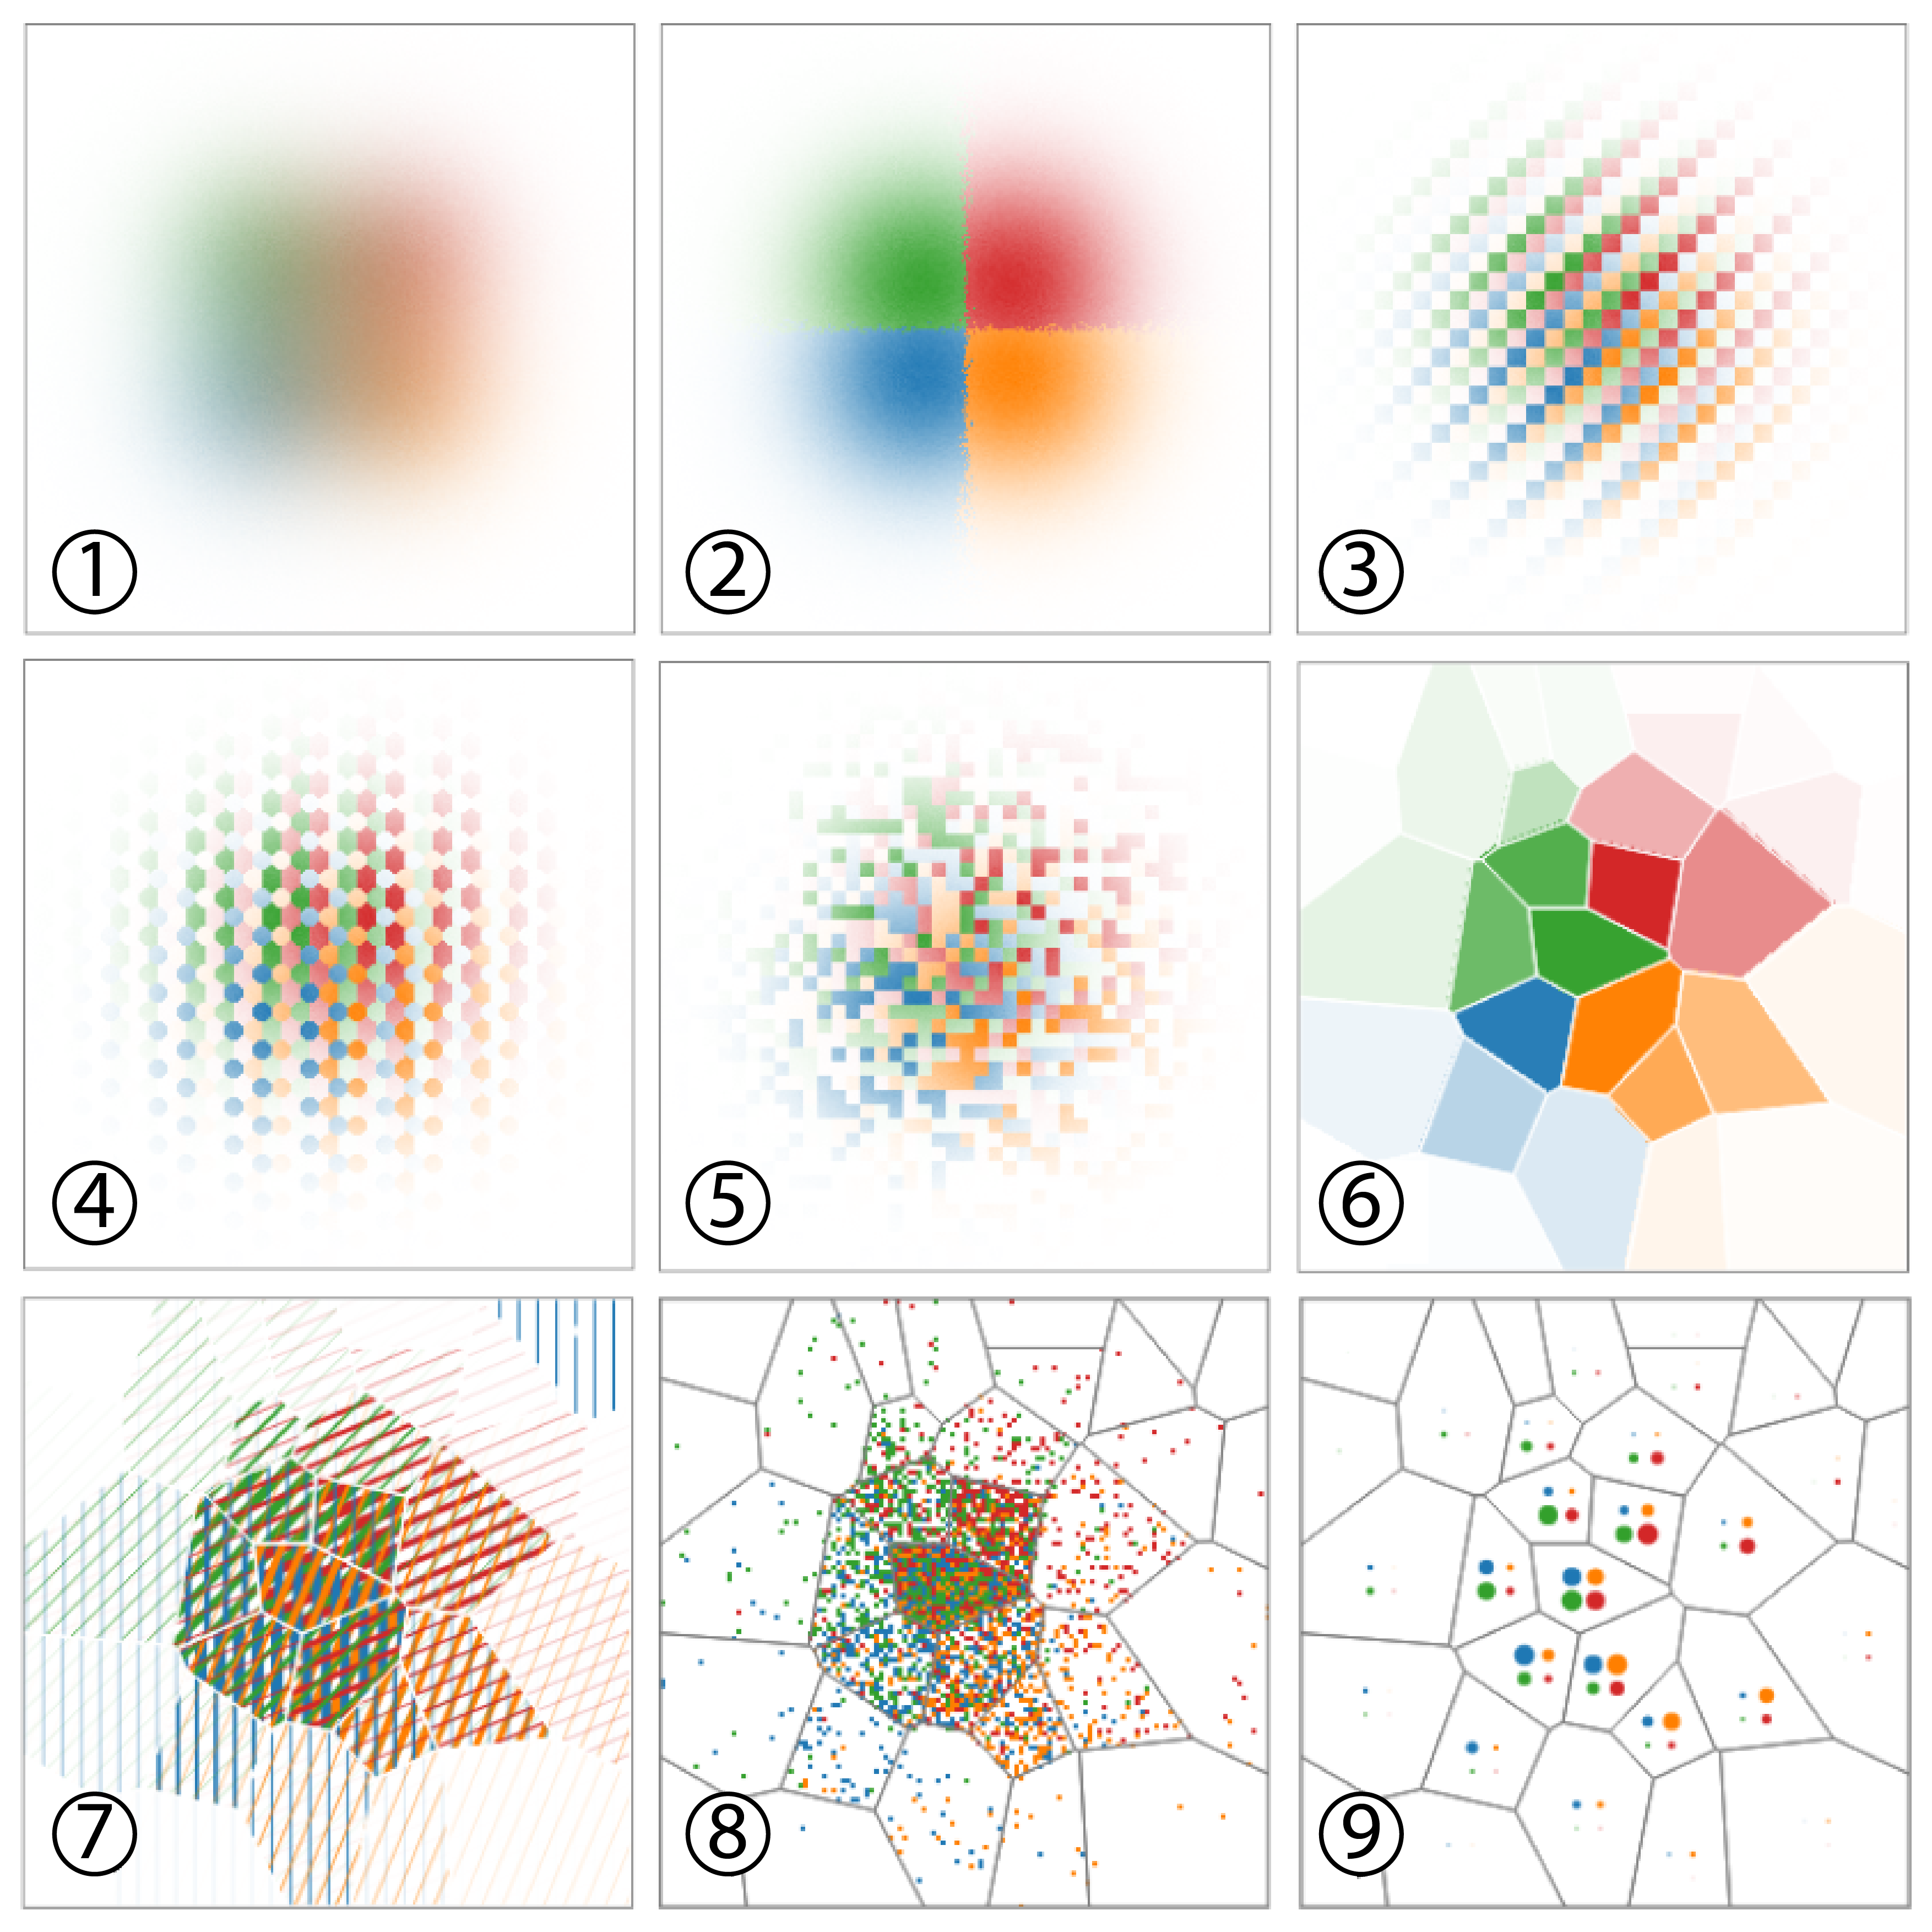
\includegraphics[width=\columnwidth]{./figures/results}
	\caption{A few results generated from the Class Buffer model. 1. Blending of the density maps. 2. winner-takes-all approach. The class with the highest count is chosen. 3. - 5. Three different weaving patterns. 3. and 4. are regular patterns, 5. is an irregular weaving pattern. 6. - 9. Uses rebinning (binning and aggregation over the density maps) with tiles produced by a random Voronoi pattern. 6. Shows the highest count in the tile, 7. Shows hatching, 8. shows a dot density plot, 9. Shows a punch card.\\\textcopyright~Extracted from \textit{A Declarative Rendering Model for Multiclass Density Maps} and digitally edited, Jo et al.,~\cite{jo2019declarative}}\label{fig:mdm-results}
\end{figure}

\begin{figure*}
	\centering
	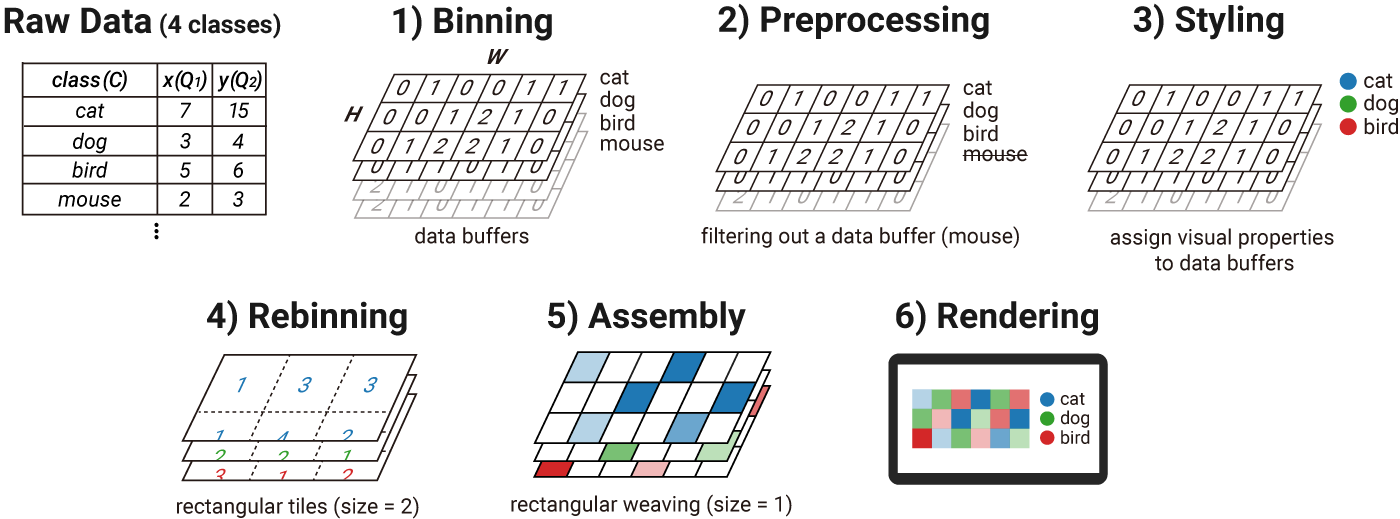
\includegraphics[width=0.85\textwidth]{./figures/Multiclass_Density_Maps-10}
	\caption{The six stages of the Class Buffer model. First binning, the data is split into as many data buffers as tables.$\star$ Second the preprocessing, like gaussian smoothing.$\bullet$ Third styling where the data buffers are assigned i.e. colors.$\bullet$ Fourth rebinning where the classes get partitioned into tiles, aggregated and normalized.$\bullet$ Fifth the assembly where tiles and normalized counts are turned into a single density map.$\bullet$ Sixth the rendering of the data, here legends axis and landmarks etc. are added for better understanding of the visualization.$\bullet$\\$\star$: Done in the back-end.$\bullet$: Done in the front-end. \textcopyright~Extracted from \textit{A Declarative Rendering Model for Multiclass Density Maps}, Jo et al.,~\cite{jo2019declarative}}\label{fig:mdm-stages}
\end{figure*}

The Class Buffer model is implemented to use the JSON data-interchange format. It defines an expressive visualization grammar for multiclass density maps, the specification of this grammar can be seen in Listing~\ref{lis:specs}. The Class Buffer model is based on the Class Buffer idiom~\cite{chen2018using} as the primary building block.
The implementation of the Class Buffer model from Jo et al. consists of six stages, that are apportioned to either the back-end that is processing much of the data or the front-end of the system displaying the data. This approach comes from the advantages of the specification, where tasks can easily be implemented on both sides of modern web applications. The back-end is responsible and capable of doing larger calculations and the front-end is dedicated to filtering, styling and displaying the data. The six stages used in the model can be seen in Figure~\ref{fig:mdm-stages} and are described as follows:

\begin{enumerate}[leftmargin=*]
	\setlength\itemsep{0.1em}
	\item \textbf{Binning.} Data that is given into the system is divided into data buffers where the number of data buffers corresponds to the number of classes in the data. A data buffer can be understood as a 2D histogram that counts the occurrence of a data case and groups those belonging together. This binning is implemented in the backend of the system because it consists of only semantic calculations and no styling. The backend will transfer the data buffers to the front-end where the second and following steps will take place.\\The main goal of doing this step on the back-end side is to enable the rendering to happen in interactive time~\cite{jo2019declarative} and because this step has to be done generally only once for the lifecycle of a map. By doing so the model supports stationary as well as handheld devices and their respective computational power.
	\item \textbf{Preprocessing.} When the data buffers get passed to the front-end of the application a preprocessing operation is realized. This preprocessing is most often a gaussian smoothing over each buffer individually. Smoothing allows the elimination of problems with excessive variability in the summaries~\cite{wickham2013bin}.\\Data can likewise be filtered by different properties and criteria that should be left out of the rendering process. Combinations of different data buffers can moreover be created. Because of this filtering and combining data into mixed data buffers the preprocessing step is done in the front-end to eliminate expensive round trips when filters change.
	\item \textbf{Styling.} The first styling step performed is a transformation from data buffers to class buffers. Class buffers represent the same separated data as data buffers but with additional information such as class specific color, hatching angle or scale.\\These visual properties are specified on the front-end using the grammar of the Class Buffer model, as described by Jo et al.~\cite{jo2019declarative} can be seen in Listing~\ref{lis:specs}.
	\item \textbf{Rebinning.} The front-end then partitions the class buffers, that is divided into grids, into tiles. These can be equidistant partitions of the two dimensional domain that the data resides in, but also a more irregular divided separation of space like a Voronoy separation. An important property is that the tiling is defined so that there is no overlapping within them. Additionally an aggregated count is computed for each class and stored in a data vector. This aggregation is all pixels from class \textit{i} that belong to the tile \textit{t}. It is afterwards normalized to a value between 0 and 1 using a linear, log, square root or equi-depth histogram scale to be used in the legend.
	\item \textbf{Assembly.} Tiles and normalized data vectors are turned into a single density map image. This step adds more styling to the process, like an alpha channel, and different approaches to unify the maps are possible, namely, masking, mixing, hatching, and generating glyphs based on the aggregated count described below.\\\textbf{Masking} is the process where a mask is assigned to each class buffer. This mask is a grid of the same size as the original grid and is defined such that the sum of every mask grid equals 1 for each pixel. Then each tile is rendered for each class buffer with a uniform color previously assigned in the styling stage and the corresponding opacity value of the normalized count stored in the data vector. The resulting image is then alpha-blended using the opacity values stored in the mask. This approach is used for the weaving pattern that can be seen in Figure~\ref{fig:mdm-results} in example 3 and 4.\\The \textbf{Mixing} operation on the other hand combine tiles by blending them. The main goal is to receive a resulting image that is similar to the one generated by masking but with colors that are blended across the entire tile instead of being masked. Different mixing methods can be used, in example \textit{additive mixing} sums each RGB channel of the colors, thus generating brighter colors as \textit{multiplicative mixing}, which generates darker colors for high density regions. Additionally, it is possible to take an \textit{winner-takes-all} or \textit{loser-takes-all} approach where either the class with the highest or lowest count is chosen.\\Tiles can furthermore be rendered by using the \textbf{hatching} operation, which fills each tile with evenly spaced lines. Typically the line thickness encodes the normalized count, while the line orientation encodes the class. The hatches can be combined by stacking them side by side within each or by superimposing them, like in Figure~\ref{fig:mdm-results}, example 7.\\A more conventional pipeline is \textbf{glyph generation} to visualize the previously processed data. Glyphs are miniature visualizations that are used to encode the normalized counts of the data and are typically rendered in the center of the tile, like in Figure~\ref{fig:mdm-results}, in example 8 and 9. The position can be slightly moved to make space for glyphs from other classes. This can result in visualizations like a punch card or the mixture of bar chart and density map where each tile in the visualization holds a bar chart indicating the normalized value of the data.\\Jo et al.~\cite{jo2019declarative} compute the position of the glyph as the largest rectangle in polygon for each tile and place the glyph in the middle of this rectangle. This assembly step might be the most comprehensive step of the Class Buffer model but it is optional as well. When no assembly operation is specified, each tile is rendered using a uniform translucent color, and the process outputs multiple density map images instead of a single one, leaving the conflict resolution to the final rendering stage.
	\item \textbf{Rendering.} The final step shows the single density map on the medium the user desires, either stationary or handheld devices, such as mobile phones. The background color of the plot defines the lower end of the color scale used in the visualization. For example, a white background will result in a color scale where white is indicating the lowest, or zero density. Black backgrounds will produce the same effect but might have other (dis-)advantages. The background does not have to be of uniform color but can also show cartographic or other information.\\In this stage a variety of helping decorations and annotations can be added, i.e. landmarks and axes, to make the visualization easier to understand by the viewer and a legend can be added to complete the visualization process.
\end{enumerate}

\blfootnote{The implementation form Jo et al. is available, with example datasets, at \url{https://github.com/e-/Multiclass-Density-Maps} and examples can additionally be explored at \url{https://jaeminjo.github.io/Multiclass-Density-Maps/}.}

The Class Buffer model is implemented in TypeScript, a strongly typed language that can be transpiled into JavaScript, which runs in every modern browser as basis of the dynamic web.
Additionally, the implementation relies on the D3 library for contours and cartographic projections.
Interpreting a specification takes between a few hundred milliseconds to one second depending on the complexity of the operations to perform~\cite{jo2019declarative}, not counting the time to transfer the data, including data buffers. 

In the implementation of the class buffer model, glyphs can be specified in Vega-Lite~\cite{satyanarayan2016vega}, a high-level JSON grammar for interactive graphics. It provides a concise JSON syntax for rapidly generating visualizations to support analysis.

Tiles can be defined based on geometrical primitives or using the URI of a TopoJSON~\cite{online:topojson} specification to define geographic administrative boundaries. TopoJSON is an extension of GeoJSON that encodes topology. Rather than representing geometries discretely, geometries in TopoJSON files are stitched together from shared line segments. TopoJSON eliminates redundancy, allowing related geometries to be stored efficiently in the same file.

Changing a specification and reinterpreting data is generally a lot quicker as information isn't changed. Intermediate operations, such as rebinning, can be cached if the tiling is not changed, which is common for geographical maps~\cite{jo2019declarative}.
Tile glyphs are rendered using Vega-Lite~\cite{satyanarayan2016vega}.

% \begin{minipage}[0mm]{\columnwidth}
\begin{lstfloat}
	\small{
		\begin{lstlisting}[caption={Syntax of Class Buffer specifications. Different TypeScript notations show the required JSON fields for the model to interpret the data in the minimal way~\cite{jo2019declarative}. Fields denoted by questionmarks can be omitted.},captionpos=b,label=lis:specs]
{"description"?: <string>,
"background"?: <Color>,
"data": {"url": <url> | "dataSpec": <DataSpec>},
"smooth"?: {"radius": <number>},
"reencoding"?: {
  "label"?: <LabelSpec>, "color"?: <ColorSpec>,
  "hatching"?: <HatchingSpec>
},
"rescale"?: {
  "type": "linear" | "log" | "pow" | 
          "sqrt" | "cbrt" | "equidepth",
  "rebin"?: {
      "type": "none" | "square" | "rect" | "topojson" | 
              "voronoi",
      "aggregation": "mean" | "max" | "sum" | "min" | 
              "density",
      "width"?: <number>, "height"?: <number>,
      "size"?: <number>, "topojson"?: <TopoJSONSpec>,
      "url"?: <string>, "feature"?: <string>,
      "points"?: <Point[]>, "stroke"?: <Color>
  },
  "compose"?: {
    "mix": "none" | "invmin" | "mean" | "max" | "blend" | 
           "weavingrandom" | "weavingsquare" | 
           "weavinghex" | "weavingtri" | "propline" | 
           "hatching" | "separate" | "glyph" | 
           "dotdensity" | "time",
    "mixing"?: "additive" | "subtractive" | 
               "multiplicative",
    "size"?: <number>, "widthprop"?: <string|number>,
    "colprop"?:<boolean>, "order"?: <number[]>,
    "glyphSpec"?: <GlyphSpec>, "interval"?: <number>
  },
  "levels"?: <number>
},
"contour"?: {
  "stroke": <number>, "lineWidth"?: <number>,
  "values"?: <number[]>, "blur"?: <number>
},
"legend"?: <LegendSpec>, "stroke"?: <StrokeSpec>,
"axis"?: <AxisSpec>}
\end{lstlisting}
	}
\end{lstfloat}

\subsection{Benefits of the Class Buffer model}
The Class Buffer model is more scalable over the three facets, data size, perceptual processing, and computation speed when compared with other frameworks for visualizing large maps~\cite{jo2019declarative}. This is largely due to the separation of computational tasks between the back-end and the front-end in the implementation.
The back-end side computes density maps, which will result in proportional computation time in relation to the number of points.
Once this expensive computation is done, the visualizations offered by the model can be used to explore the data at 'interactive' speed, regardless of the size of the original data.
Jo et al.~\cite{jo2019declarative} argue that it can be about millions, billions, or any higher scale of data points.

Other visualization libraries compute the aggregation and the visualization together, needing a time proportional to the number of points to generate a new visualization and require expensive round-trips from the back-end to the browser. Abstract Rendering~\cite{cottam2013overplotting, cottam2014abstract} performs the binning operations in complex buffers that are configured early before their contents are computed.
Once computed, most of the rendering has to be performed in the back-end as well because the composite structure at each bin is structured in a way that a transparent transmission to a front-end for easy visualization becomes impractical. Each modification of the pipeline requires an expensive recomputation starting at the binning stage, requiring the handling of the whole dataset.

By contrast, the Class Buffer model receives the raw unsmoothed density map and can apply a smoothing kernel to it at its first stage. According to Wickham~\cite{wickham2013bin}, applying the smoothing to the binned data produces very similar results than applying it before binning, with a substantial performance improvement~\cite{wand1994fast}. Compared with Wickham’s BSS model~\cite{wickham2013bin}, the Class Buffer model provides a richer set of visualization options, but less statistical operations at the prebinning stage. This is because the BSS model does not manage multiclass data.

% Copmposing multiple classes from density maps is understandable since densities are directly comparable, but with more complex statistics such as average, variance, or higher-order moments, the interpretations of the class combinations are challenging.

\subsection{Interactive Data Exploration}

The Class Buffer model uses 2D histograms, calculated from data buffers, as data sources. This provides the model with the ability to abstract the underlying computation of large-scale data~\cite{jo2019declarative}.
When the dataset is filtered by a new dimension, the data buffers should be invalidated and recomputed. Because of the changes in the filtering all binning could be changed, which results in the need for completely new data aggregated by different properties. 
In interactive exploration with multidimensional data, this would be a frequent case, and modern data structures~\cite{lins2013nanocubes, liu2013immens} have been proposed to speed up the recomputation. The Class Buffer model naturally lends itself to working with those optimized data structures through the transfer of \textit{abstract} data buffers between the front- and back-end of the system. The model uses this method in order to facilitate a dynamic change of visualization types in real time on all devices. The user can, by using this system, view multiple variants of visualizations for the same group of data bins.\\ 
In addition, the ProgressiVis toolkit~\cite{fekete2016progressive} already transfers data buffers of progressively aggregated data to its front-end, which can be used with the Class Buffer model.

% \textcolor{red}{\lipsum[2]}

\subsection{Limitations}

A wide variety of visualizations, suited to complex tasks, can be created using the Class Buffer model. These visualizations show the complex data in a way that the viewer might comprehend coherences more easily and with less cognitive effort than visualizations created by hand. They almost always need additional information to be fully comprehensible, such as landmarks, points of interest, and marks of outliers. The depiction, because of the binning, masking and mixing, additionally needs a legend.
Landmarks for maps include important locations and names, sometimes additional shapes to add context, such as rivers or points of interest. Landmarks for scatterplots and multidimensional projections include location of interesting points.
For example, in publication data, highly cited publications or authors can be used as landmarks.
All these additional guides should be combined and added to the image at the rendering stage.

The Class Buffer model can replicate several techniques used to visualize multiclass density maps, but it does not offer guidance on their best use. 
By providing this implementation Jo et al.~\cite{jo2019declarative} enable the visualization community to continue researching multiclass density maps, opening up a new area of scalable visualization. 


\section{Discussion}

The Class Buffer model is more scalable over the three facets compared to other frameworks for viewing large scale data: data size, perceptual processing, and computation speed.
The enhanced perceptual processing arises from the broad spectrum of visualization methods that can be generated for density maps of multiple classes.
The model on the other hand does not guide users in a very good way. The challenges of understanding and using the different visualization methods have to be further investigated.
Multiclass density maps often have the disadvantage of obfuscating information when mixing or masking is introduced but they can also display more data classes that can be easily shown when using dot density maps. Different classes intersect, overlap and interfere with each other and by this make it hard to understand these kind of maps.
There are a multitude of visualization results that appear to visualize the data in a reasonably good way, but often the results obfuscate the data in a way that makes it hard to comprehend the full scope of the information present. In example the data that gets presented often mix or mask certain areas of interest. This results in clusters being mixed with neighboring clusters and thus losing the possibility to show the true amount of datapoints present in one group. Additionally outliers get overlaid by datapoints from other groups or get scaled down to an extend that they cannot be perceived at all when using the visualization methods provided by the Class Buffer model implementation, this effect can be seen in Figure~\ref{fig:outliers}.

\begin{figure}
	\centering
	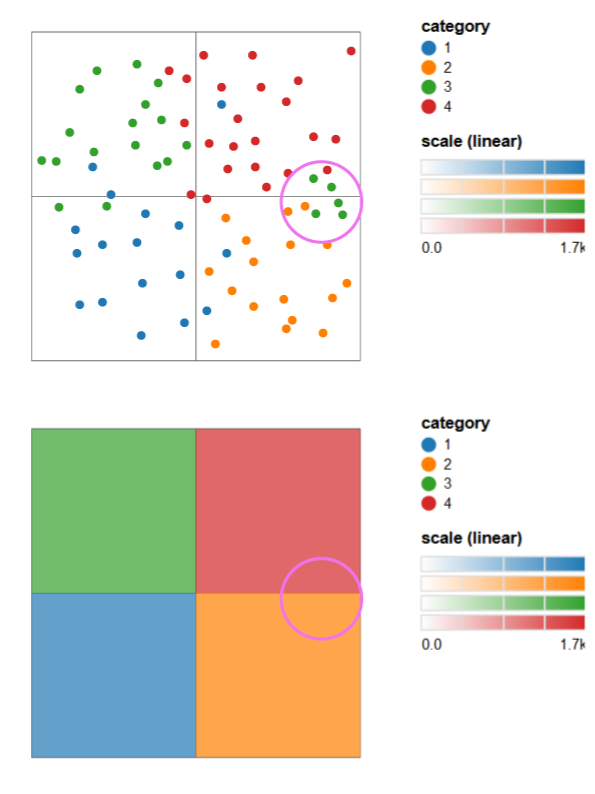
\includegraphics[width=0.85\columnwidth]{./figures/outliers}
	\caption[outliers]{A portrayal of the effect present when masking classes with other classes. In the top picture the data is visualized as a standard 2D scatterplot. The group of outliers get lost in the visualization process, which can be seen in the bottom picture.}~\label{fig:outliers}
\end{figure}

The Class Buffer model implemented by Jo et al. uses different approaches to display data but just few of them result in classical density maps~\cite{jo2019declarative}, some also arouse the impression of dot density maps with different tiling or aggregation.
A density map can be more challenging to comprehend when used in the wrong context or when implemented wrong or without an appropriate understanding of the field.\\It is thus essential to improve the presented method further. This could be done by enhancing the visual separation with additional options or by implementing an expressive guiding toolbox or some other kind of guideline. By providing the user with the basic tools to generate multiclass density maps the first step has been taken.

% \textcolor{red}{\lipsum[1]}

% \improvement{Clusters are seperable, outliers get lost}


\section{Conclusion}\label{conclusion}

In the future, as well as today, fault-proneness estimation and prediction could play a key role in software product quality control.  In this area, much effort has been invested in defining metrics and identifying models for system evaluation, object-oriented models as well as others.  Using these metrics to assess which parts of the system are more fault-proneness is of primary importance, as summarized in this paper.
Much work has concentrated on how to select the software metrics that are most likely to indicate fault-proneness. 

In the field of software evolution, metrics can be used for identifying stable or unstable parts of software systems.

Moreover the question is, what can really prevent faults in the later used system beforehand?

If you take up the other software trends of development mentioned at the beginning, it becomes clear that they are all connected in a certain way. The fault-proneness and the maintenance grow with increasing complexity.Ensuring security and quality always involves a number of features.

%- summarize discussion and results; name important metrics/properties that should stay in mind after reading this

%- what can reduce the fault-pron in software development

%- outlook future work (future work wäre größere systeme anschauen und testen auf faulty classes und metriken testen an sich)

%- This paper discussed the concept of fault proneness using the example of object-oriented programming and design metrics, which means that for the most part the results can only be transferred to the object-oriented context.


%- final catch and the link to the superordinate context (research trends in software technology); link to introduction and motivation

%wie in related work aufgezeigt die flexible metrics die können als ausblick hilfreich sien wenn sich der kontexxt leicht ändert

%% if specified like this the section will be ommitted in review mode
% \acknowledgements{
% The authors wish to thank A, B, C. This work was supported in part by
% a grant from XYZ.}

\bibliographystyle{abbrv}
%%use following if all content of bibtex file should be shown
% \nocite{*}
\bibliography{template}

% \newpage
% \listoftodos[Notes]
\end{document}
